%\renewcommand{\thefootnote}{\arabic{footnote}}
\chapter{TINJAUAN PUSTAKA}
\label{BAB2:tinjauan}

Manfaatkan penggunaan perintah \verb|\label{}| untuk menjadikan suatu bab atau subbab sebagai acuan. Untuk mengacu ke bab atau subbab itu maka gunakan perintah \verb|\ref{}|. Sebagai contoh, Bab \verb|\ref{BAB1:pendahuluan}| akan menghasilkan: Bab \ref{BAB1:pendahuluan}. Teknik yang sama juga bisa digunakan untuk mengacu ke suatu gambar atau tabel. Sebagai contoh, Gambar~\ref{fig:arsitektur} menunjukkan arsitektur dari blok \textit{Residual Networks} (ResNet).
\begin{figure}[h]
    \centering
    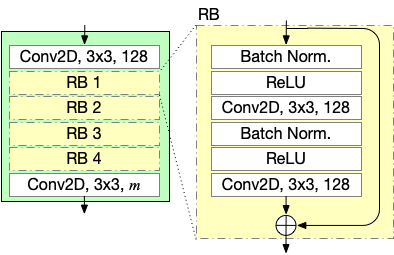
\includegraphics[scale=0.5]{BAB-2/resnet receiver.png}
    \caption{Arsitektur Blok ResNet}
    \label{fig:arsitektur}
\end{figure}

Salah satu cara untuk membuat tabel, seperti yang ditunjukkan pada Tabel~\ref{tab:test}, adalah dengan menggunakan \verb|longtblr| \citep{tabularray}.

\begin{table}[h]
    \centering
    \caption{Tabel dengan tblr}
    \label{tab:my_label}

    \begin{tblr}{lccr}
    \hline
    Alpha & Beta & Gamma & Delta \\
    \hline
    Epsilon & Zeta & Eta & Theta \\
    \hline
    Iota & Kappa & Lambda & Mu \\
    \hline
    \end{tblr}
\end{table}

\begin{longtblr}[
  caption = {Tabel yang panjang},
  label = {tab:test}
]{
  colspec = {|XX[4]|},
  rowhead = 1,
  hlines,
  row{even} = {gray9},
  row{1} = {olive9}
} 
No. & Kolom 1 \\
1  & blablabla \\
2  & blablabla \\
3  & blablabla \\
4  & blablabla \\
5  & blablabla \\
6  & blablabla \\
7  & blablabla \\
8  & blablabla \\
9  & blablabla \\
10  & blablabla \\
11  & blablabla \\
12  & blablabla \\
13  & blablabla \\
14  & blablabla \\
15  & blablabla \\
16  & blablabla \\
17  & blablabla \\
18  & blablabla \\
19  & blablabla \\
20  & blablabla \\
21  & blablabla \\
22  & blablabla \\
\end{longtblr}

\begin{longtblr}[
  caption = {Tabel Dataset Jawaban Mahasiswa},
  label = {tab:test2},
]{
  colspec = {|c|XX[1]|c|},
  rowhead = 1,
  hlines,
  row{even} = {gray9},
  row{1} = {olive9},
  % |l|,
} 
No & Nama Kolom            & Tipe Data \\  
1  & Nim                   & ordinal   \\  
2  & Jawaban pertanyaan 1  & String    \\  
3  & Jawaban pertanyaan 2  & String    \\  
4  & Jawaban pertanyaan 3  & String    \\  
5  & Jawaban pertanyaan 4  & String    \\  
6  & Jawaban pertanyaan 5  & String    \\  
7  & Jawaban pertanyaan 6  & String    \\  
8  & Nilai No 1            & nominal   \\  
9  & Nilai No 2            & nominal   \\  
10 & Nilai No 3            & nominal   \\  
11 & Nilai No 4            & nominal   \\  
12 & Nilai No 5            & nominal   \\  
14 & Total Nilai           & nominal   \\  
\end{longtblr}